%%%%%%%%%%%%%%%%%%%%%%%%%%%%%%%%%
%
%       EXERCÍCIO
%
%%%%%%%%%%%%%%%%%%%%%%%%%%%%%%%%%

\ifdefstring{\atividade}{prova}{%
    \ifdefstring{\modo}{objetivo}{%
        \renewcommand{\valorquestao}{\ValorQObj\ ponto}
    }{%
        \renewcommand{\valorquestao}{\ValorQDisc\ pontos}
    }%
}%

\begin{exercicioBanco}[\valorquestao]
Das figuras a seguir, indique aquela que representa o gráfico de uma função real \(f: [a,b] \to \bbR\), onde \(a, b \in \bbR\).

% Define as alternativas
\newcommand{\alternativas}{%
    \begin{center}
        \begin{tabularx}{\textwidth}{XXX}
            \hspace{40pt} (a) & \hspace{40pt} (b) & \hspace{40pt} (c) \\[5pt]
            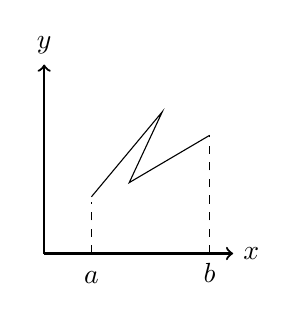
\begin{tikzpicture}[scale=0.6]
                \draw[->,thick] (0,0)--(4,0) node[right]{$x$};
                \draw[->,thick] (0,0)--(0,4) node[above]{$y$};
                \draw[dashed] (1,0)--(1,1.1);
                \draw[dashed] (3.5,0)--(3.5,2.5);
                \draw (1,1.2)--(2.5,3)--(1.8,1.5)--(3.5,2.5);
                \draw node[below, yshift=-3pt] at (1,0) {\(a\)};
                \draw node[below] at (3.5,0) {\(b\)};
            \end{tikzpicture}
            &
            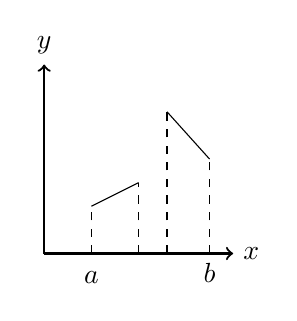
\begin{tikzpicture}[scale=0.6]
                \draw[->,thick] (0,0)--(4,0) node[right]{$x$};
                \draw[->,thick] (0,0)--(0,4) node[above]{$y$};
                \draw[dashed] (1,0)--(1,1);
                \draw[dashed] (3.5,0)--(3.5,2);
                \draw (1,1)--(2,1.5);
                \draw[dashed] (2.6,0)--(2.6,3);
                \draw (2.6,3)--(3.5,2);
                \draw[dashed] (2,0)--(2,1.5);
                \draw node[below, yshift=-3pt] at (1,0) {\(a\)};
                \draw node[below] at (3.5,0) {\(b\)};
            \end{tikzpicture}
            &
            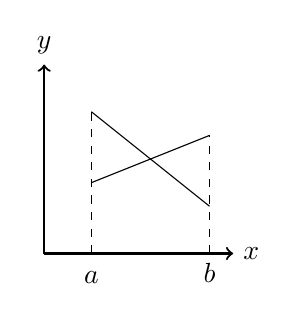
\begin{tikzpicture}[scale=0.6]
                \draw[->,thick] (0,0)--(4,0) node[right]{$x$};
                \draw[->,thick] (0,0)--(0,4) node[above]{$y$};
                \draw[dashed] (1,0)--(1,3);
                \draw[dashed] (3.5,0)--(3.5,2.5);
                \draw (1,3)--(3.5,1);
                \draw (1,1.5)--(3.5,2.5);
                \draw node[below, yshift=-3pt] at (1,0) {\(a\)};
                \draw node[below] at (3.5,0) {\(b\)};
            \end{tikzpicture}
            \\[13pt]
            \hspace{40pt} (d) & \hspace{40pt} (e) & \\[5pt]
            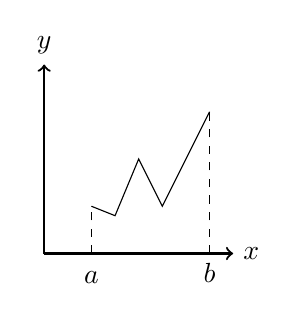
\begin{tikzpicture}[scale=0.6]
                \draw[->,thick] (0,0)--(4,0) node[right]{$x$};
                \draw[->,thick] (0,0)--(0,4) node[above]{$y$};
                \draw[dashed] (1,0)--(1,1);
                \draw[dashed] (3.5,0)--(3.5,3);
                \draw (1,1)--(1.5,0.8)--(2,2)--(2.5,1)--(3.5,3);
                \draw node[below, yshift=-3pt] at (1,0) {\(a\)};
                \draw node[below] at (3.5,0) {\(b\)};
            \end{tikzpicture}
            &
            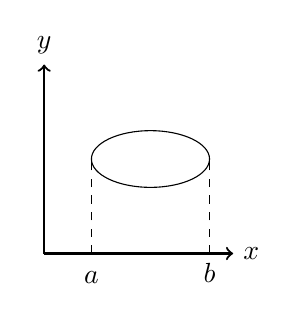
\begin{tikzpicture}[scale=0.6]
                \draw[->,thick] (0,0)--(4,0) node[right]{$x$};
                \draw[->,thick] (0,0)--(0,4) node[above]{$y$};
                \draw[dashed] (1,0)--(1,2);
                \draw[dashed] (3.5,0)--(3.5,2);
                \draw (2.25,2) ellipse (1.25 and 0.6);
                \draw node[below, yshift=-3pt] at (1,0) {\(a\)};
                \draw node[below] at (3.5,0) {\(b\)};
            \end{tikzpicture}
            &
        \end{tabularx}
    \end{center}
}

% Define a resposta correta
\newcommand{\resposta}{D}

% Lógica condicional para exibição
\ifdefstring{\atividade}{lista}{%
    \alternativas
    \vspace{0.5em}
    
    \noindent\textbf{Resposta:} letra \textbf{\resposta}.
}{%
    \ifdefstring{\modo}{objetivo}{%
        \alternativas
    }{%
        % modo = discursiva → não mostra alternativas
    }
}
\end{exercicioBanco}

